\documentclass[12pt, a4paper]{article}

\usepackage{amssymb}
\usepackage{multicol}
\usepackage{enumerate}
\usepackage[top=5em, bottom=5em, left=5em, right=5em]{geometry}
\usepackage{listings}
\usepackage{tikz}
\usetikzlibrary{positioning}

\setlength\parskip{1em}
\setlength\parindent{0em}

\title{Assignment}

\author{Hendrik Werner s4549775}

\begin{document}
\maketitle

This was done in collaboration with Constantin Blach (s4329872).

\section{} %1
Initial state:

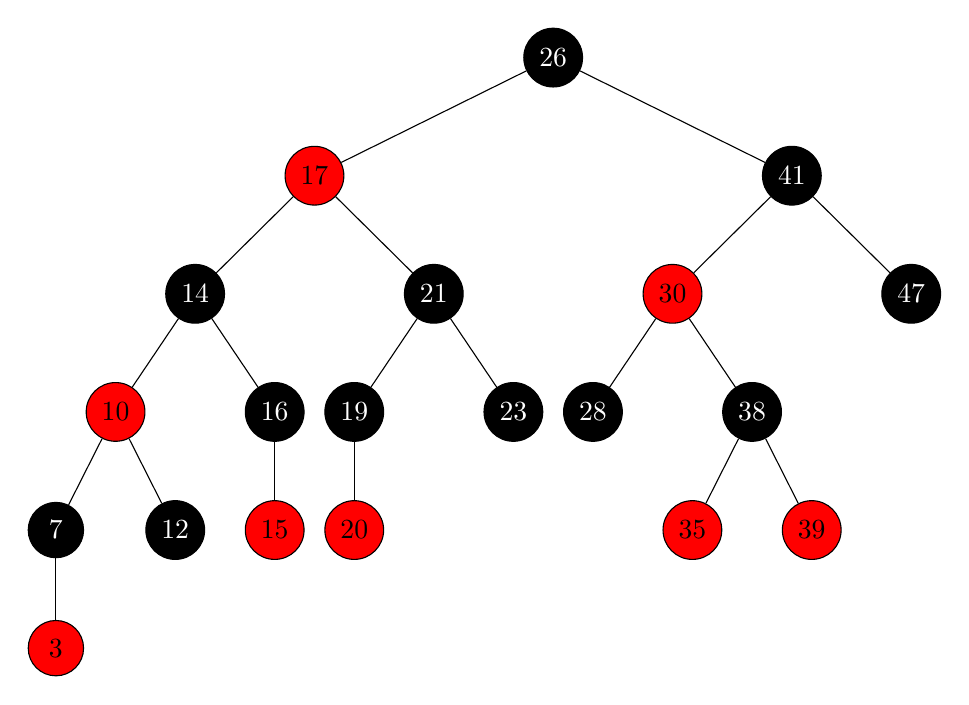
\begin{tikzpicture}[
	every node/.append style={minimum width=2em}
	,level/.style={sibling distance=.5\linewidth/#1}
	,b/.style={circle, draw, fill=black, text=white}
	,r/.style={circle, draw, fill=red}
]
	\node [b] (A) {26}
		child {
			node [r] (B) {17}
			child {
				node [b] (D) {14}
				child {
					node [r] (H) {10}
					child {
						node [b] (N) {7}
						child {
							node [r] (T) {3}
						}
					}
					child {
						node [b] (O) {12}
					}
				}
				child {
					node [b] (I) {16}
					child {
						node [r] (P) {15}
					}
				}
			}
			child {
				node [b] (E) {21}
				child {
					node [b] (J) {19}
					child {
						node [r] (Q) {20}
					}
				}
				child {
					node [b] (K) {23}
				}
			}
		}
		child {
			node [b] (C) {41}
			child {
				node [r] (F) {30}
				child {
					node [b] (L) {28}
				}
				child {
					node [b] (M) {38}
					child {
						node [r] (R) {35}
					}
					child {
						node [r] (S) {39}
					}
				}
			}
			child {
				node [b] (G) {47}
			}
		}
	;
\end{tikzpicture}

When adding the key 36 it is inserted at the following position:

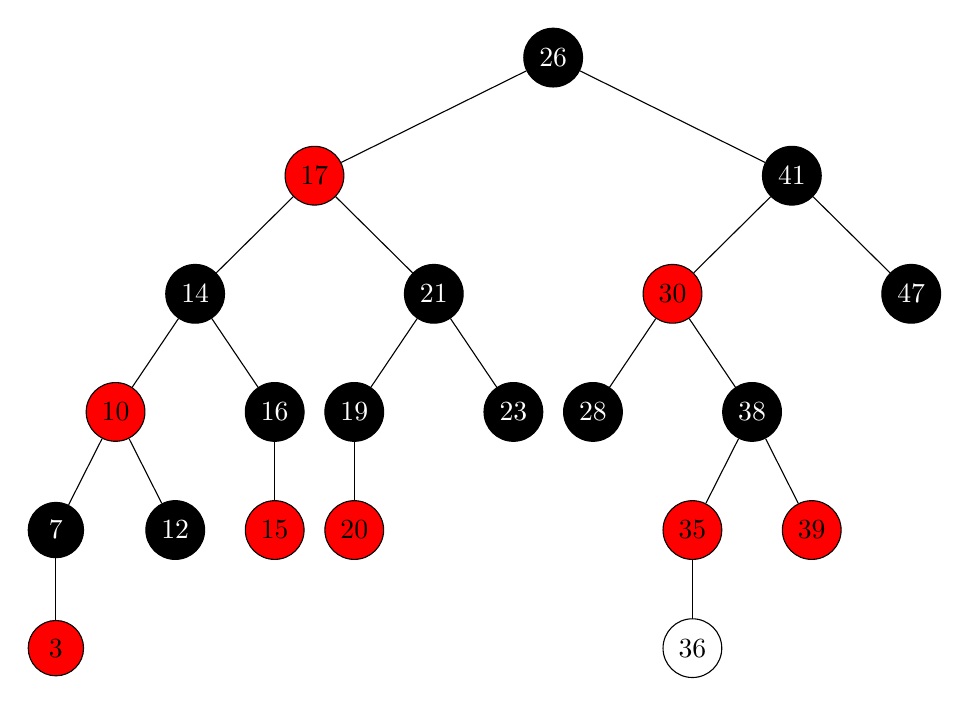
\begin{tikzpicture}[
	every node/.append style={minimum width=2em}
	,level/.style={sibling distance=.5\linewidth/#1}
	,b/.style={circle, draw, fill=black, text=white}
	,r/.style={circle, draw, fill=red}
]
	\node [b] (A) {26}
		child {
			node [r] (B) {17}
			child {
				node [b] (D) {14}
				child {
					node [r] (H) {10}
					child {
						node [b] (N) {7}
						child {
							node [r] (T) {3}
						}
					}
					child {
						node [b] (O) {12}
					}
				}
				child {
					node [b] (I) {16}
					child {
						node [r] (P) {15}
					}
				}
			}
			child {
				node [b] (E) {21}
				child {
					node [b] (J) {19}
					child {
						node [r] (Q) {20}
					}
				}
				child {
					node [b] (K) {23}
				}
			}
		}
		child {
			node [b] (C) {41}
			child {
				node [r] (F) {30}
				child {
					node [b] (L) {28}
				}
				child {
					node [b] (M) {38}
					child {
						node [r] (R) {35}
						child {
							node [circle, draw] (U) {36}
						}
					}
					child {
						node [r] (S) {39}
					}
				}
			}
			child {
				node [b] (G) {47}
			}
		}
	;
\end{tikzpicture}

We could either color it black, which would violate property 5 ("For each node, all paths from node to descendant leaves contain same number of black nodes"): The path $38 \rightarrow 39 \rightarrow nil$ has a black heigth of 1 while $38 \rightarrow 35 \rightarrow 36 \rightarrow nil$ has a black height of 2.

Alternatively we could color it red which would violate property 4 ("If a node is red, then both its children are black.") because 36 is a child of 35 and 35 is red.

\section{} %2

The maximum height of a red-black tree is $2bh$, where $bh$ is the black height of the root node. Thus the maximum height of a red-black tree with $bh = k$ is $2k$. The leaf node $nil$ is always present so we need to add it as well, and subtract one from the exponent because the leaf node exists only once.

We can calculate the maximum number of nodes which is $2^{2k - 1} + 1$.

\section{} %3

\begin{description}
	\item[Inserting 32]
	
\begin{tikzpicture}[
		every node/.append style={minimum width=2em}
		,level/.style={sibling distance=.5\linewidth/#1}
		,b/.style={circle, draw, fill=black, text=white}
		,r/.style={circle, draw, fill=red}
		,baseline=(A.north)
	]
		\node [b] (A) {32};
	\end{tikzpicture}

	\item[Inserting 27]
	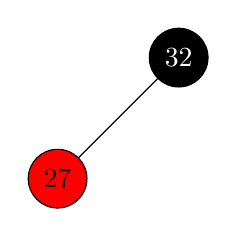
\begin{tikzpicture}[
		every node/.append style={minimum width=2em}
		,level/.style={sibling distance=.5\linewidth/#1}
		,b/.style={circle, draw, fill=black, text=white}
		,r/.style={circle, draw, fill=red}
		,baseline=(A.north)
	]
		\node [b] (A) {32}
			child {
				node [r, below left=of A] (B) {27}
			}
		;
	\end{tikzpicture}
	\item[Inserting 20]
	\item[Inserting 15]
	\item[Inserting 19]
	\item[Inserting 33]
	\item[Deleting 19]
	\item[Deleting 32]
\end{description}

\section{} %4

\section{} %5

\end{document}
